\chapter{Armonización}
\label{cap:armonizacion}

\section{¿Qué es armonizar?}
\label{sec:arm:cuestion}    

    Aunque armonizar pueda tener diversas conotaciones dependiendo del contexto, a partir de ahora, en este módulo del TFG, el término 'armonizar' se referirá específicamente a la tarea de encontrar la armonía más adecuada para una melodía dada. Es decir, buscar la mejor secuencia de acordes, según unas normas establecidas, que acompañen y enriquezcan a la melodía. Esta secuencia de acordes sería utilizada por posteriores módulos de la aplicación.

    Cabe dejar claro que, buscar 'la mejor' armonía para una melodía es algo relativo, ya que depende de la subjetividad de cada persona. Así que lo dejaremos en buscar una armonía fuertemente coherente para una melodía dada, que forme parte del espectro de soluciones razonables, ya que, por lo general, una melodía puede ser acompañada por varios conjuntos de acordes distintos.

    También comentar que, al resolver este problema, se estaría construyendo de forma implícita un analizador armónico. Si la entrada a este módulo fuese, en vez de únicamente una melodía, una canción completa, la cual contiene mucha más información, la salida esperada sería la armonía de dicha canción. Esto tiene mucha utilidad, ya que el análisis armónico es fundamental para el estudio en profundidad de una obra. La armonía conforma los cimientos de una composición musical. 

    \section{Preparativos}

    Antes de empezar con las técnicas de armonización utilizadas, falta un paso previo crucial. Y es la creación de una estructura de clases y métodos que den soporte a todo lo explicado en el apartado \ref{sec:arm:armonia}. Existen clases que abstraen lo que representa una nota musical (\ref{arm:notas_musicales}), un intervalo (\ref{sec:arm:intervalos}), una escala (\ref{sec:arm:escalas}) y la armonía de una escala (\ref{arm:armonia_escala}) tal como se ha explicado. Un acorde (\ref{sec:arm:acordes}) es respresentado también como una escala. 
    
    También es importante mostrar las respresentaciones que se están utilizando para almacenar una canción (conjunto de notas) en este módulo de la aplicación. Existen métodos para pasar de la primera representación a la segunda:

    \begin{enumerate}
        \item \textbf{Lista de notas}: es la representación estándar en este módulo de la aplicación. Se almacenan de forma desordenada diccionarios con la siguiente estructura:
        \begin{enumerate}
            \item[\textbullet] \textbf{note}: almacena el pitch MIDI (tono) de la nota. Guardar el pitch MIDI es similar a guardar la nota musical, ya que este almacena de forma implícita el nombre de la nota y su octava. Por ejemplo, calculemos a qué nota le corresponde el pitch 40:
            \begin{enumerate}
                    \item[\(\circ\)] \textbf{Nombre}: 40 mod 12 = 4, según la tabla \ref{tab:nota_pitch} a un 4 le corresponde E.
                    \item[\(\circ\)] \textbf{Octava}: 40 div 12 = 3, está en la tercera octava.
            \end{enumerate}
                       
\begin{table}[htbp]
    \centering
    \begin{tabular}{c|c}
        \textbf{Nombre} & \textbf{Pitch} \\
        \hline
        C & 0 \\
        C\# / Db & 1 \\
        D & 2 \\
        D\# / Eb & 3 \\
        E & 4 \\
        F & 5 \\
        F\# / Gb & 6 \\
        G & 7 \\
        G\# / Ab & 8 \\
        A & 9 \\
        A\# / Bb & 10 \\
        B & 11 \\
    \end{tabular}
    \caption{Relación entre cada Nota Musical y su Pitch en la Primera Octava}
\label{tab:nota_pitch}
\end{table}

        \item[\textbullet] \textbf{start\_time}: tiempo en ticks en el que empieza a sonar una nota desde que empieza la canción en el tick 0.
        \item[\textbullet] \textbf{duration}: tiempo en ticks desde que empieza a sonar la nota hasta que para.
    \end{enumerate}
    \item \textbf{Diccionario de eventos}: se almacena en cada tick clave el evento que ha ocurrido. Los ticks clave están ordenados de menor a mayor. Como tal, solo existen dos tipos de eventos: 
    \begin{enumerate}
        \item[\textbullet] \textbf{note\_on}
        \item[\textbullet] \textbf{note\_off}
    \end{enumerate}
    A cada evento viene asociado el pitch de la nota afectada. Esto puede suponer, a priori, un inconveniente, ya que, si hay dos notas del mismo pitch superpuestas en el mismo espacio de tiempo, existe una ambigüedad a la hora de saber qué evento \textit{note\_off} le corresponde a cada una. Sin embargo, esta representación se utiliza de forma temporal para facilitar la implementación de ciertos algoritmos a los cuales cuales este inconveniente no les afecta. 
    
\end{enumerate}

    Falta por explicar el concepto de tick. Un tick es la unidad simbólica mínima e indivisible que puede durar una nota. En cada canción (conjunto de notas) se debe definir el número de ticks que dura un pulso. Un pulso también se puede traducir como una negra, un beat o un step. Cuanto mayor sea el número de ticks por pulso, mayor será el número de partes en el que puedes dividir el pulso. Haciendo una analogía con la representación simbólica que se utiliza en las partituras, si los ticks por pulso son iguales a 4, en nuestra canción la semicorchea sería la representación mínima que se podría utilizar, mientras que si fueran igual a 8, la fusa sería la representación mínima (una fusa es la mitad de una semicorchea). De todas formas, lo normal es que los el número de ticks por pulso sea más alto para permitir mayor número de divisiones y combinaciones.

\section{Armonización por ventanas}\label{arm:sec:ventanas_normal}

    Este fue el primer algoritmo diseñado, el cual escalará y evolucionará en posteriores subapartados. Se basa en una idea, a priori, sencilla: dividir la canción en ventanas. Una ventana es una idea propia, y se define como conjunto de pulsos consecutivos que comprenden las notas que se hallan en dicho segmento. La idea es dividir la canción en ventanas de un determinado número de pulsos y asignar a cada una, es decir, al conjunto de notas que abarca, el acorde que mejor encaje según una heurística.

    Tanto la idea de las ventanas, como la heurística utilizada, están estrechamente relacionadas con como funcionan los compases en la música real. En castellano, se define como compás tanto a la fracción que se encuentra al principio de un pentagrama, como a cada uno de los espacios comprendidos entre las líneas (horizontales) divisorias (\ref{fig:sheet4/4}). El denominador de la fracción representa una figura musical, y cada figura musical representa un determinado número de pulsos. En este caso, el denominador es el número 4, que representa una negra, la cual dura un pulso. El numerador nos indica la cantidad de figuras, por ende, la fracción 4/4 nos está diciendo que un compás abarca 4 * 1 = 4 pulsos. 

\begin{figure}[h]
    \begin{center}
        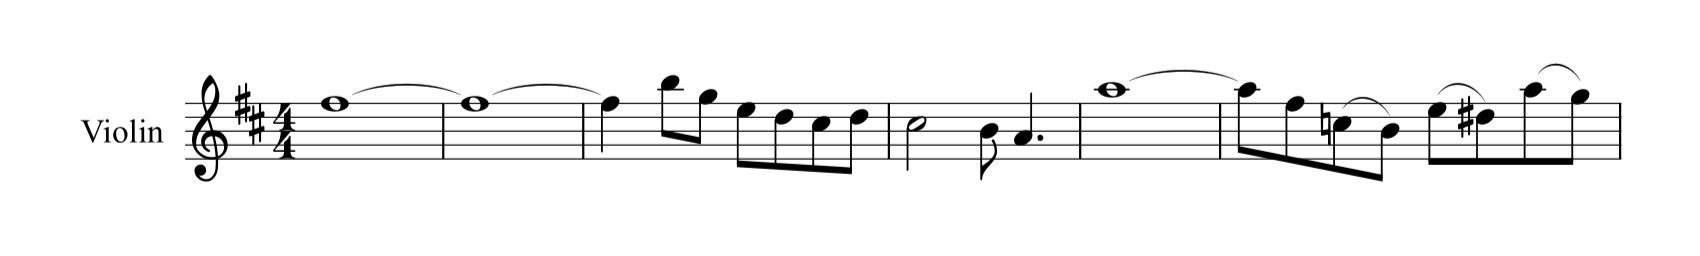
\includegraphics[scale=0.65]{Imagenes/Bitmap/partitura.png}
    \end{center}
    \caption{Partitura en 4/4}
    \label{fig:sheet4/4}
\end{figure}

    Veamos otro ejemplo con el compás 6/8 (\ref{fig:sheet6/8}). El denominador es el número 8, que representa una corchea. La corchea dura medio pulso. El númerador nos indica que en cada compás caben 6 corcheas, es decir 6 * 0.5 = 3 pulsos.

\begin{figure}[h]
    \begin{center}
        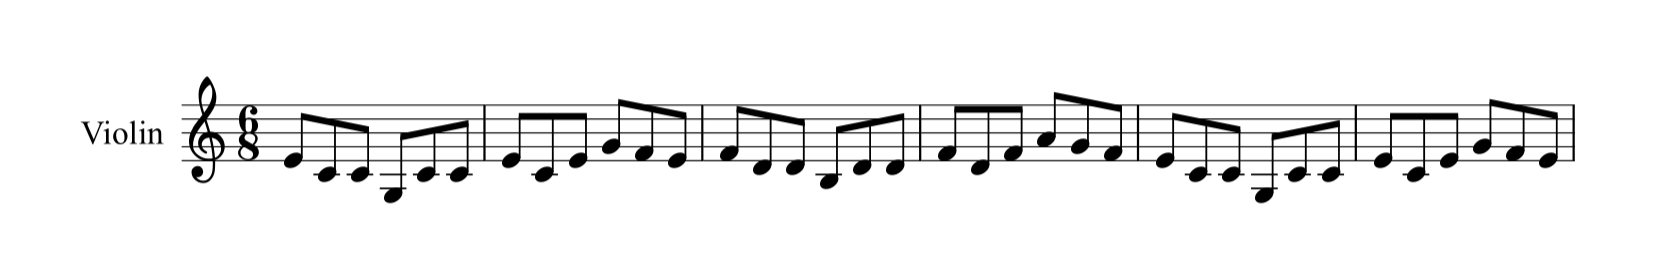
\includegraphics[scale=0.65]{Imagenes/Bitmap/partitura2.png}
    \end{center}
    \caption{Partitura en 6/8}
    \label{fig:sheet6/8}
\end{figure}

    Sabiendo esto, se puede establecer una clara analogía entre los compases y el concepto de ventana. La fracción nos indica el número de pulsos que abarca cada ventana, y las notas encerradas entre las líneas divisorias de cada compás serían las que cada ventana tiene en cuenta para elegir un acorde. 

    La idea es rellenar una lista en la que cada índice represente cada ventana. Dependiendo de cómo de larga sea una canción y cómo de grandes sean las ventanas, el tamaño de la lista variará. Cada ventana contendrá información del peso de todos los acordes que hayan sido valorados para acompañar al conjunto de notas que abarque la ventana. Se elige finalmente el acorde de mayor peso para cada ventana. Si un acorde no aparece en la lista de acordes es porque tiene peso 0, es decir, ni siquiera se ha valorado como candidato para encajar en la ventana. El peso de los acordes se calcula a partir de la heurística que se explicará a continuación.

    \label{arm:problema_acordes}
    Sin embargo, para definir el cómo se va a valorar cada acorde, se ha de elegir antes qué acordes se van a valorar. Primero se debe elegir qué tipo de acordes se quiren detectar. Por ejemplo, el conjunto de las cuatro tríadas definido anteriormente (\ref{tab:triads}). Ahora bien, como existen 12 notas musicales, se van a valorar 48 acordes diferentes por cada ventana, y eso solo teniendo encuenta 4 tipos de acordes. Dicha cifra podría escalar. A pesar de esto, el problema está no tanto en el rendimiento, sino en el hecho de que se estarían valorando acordes que contienen notas que no se encuentra en el conjunto de notas de la melodía, es decir, notas fuera de la escala, puediendo así aparecer soluciones poco deseadas. Para paliar este problema, se escogerán únicamente acordes cuyo conjunto de notas esté comprendido en la escala que forma el conjunto de notas de la melodía. Es decir, se utilizará la armonía de la escala que forma el conjunto de notas de la melodía. Esto mitiga considerablemente el problema, pero no lo llega a solucionar, además de generar otros. Estos problemas se explicarán y se intentarán solucionar en apartados posteriores, por ahora, nos sirve esta solución, ya que esto no es más que una primera versión del algoritmo que se pretende construir.

    A partir de ahora, se trabajará en términos relativos. De hecho, todo lo explicado anteriormente se ha implementado así, aunque en la explicación se haya querido abstraer. Toda la arquitectura del módulo ha sido pensada para trabajar en estos términos relativos. Eso significa que, en vez de con notas musicales, se trabajará con grados e intervalos. Esto se logra estableciendo cualquier nota del conjunto de notas de la melodía como tónica (al menos por ahora; esto podría cambiar en el futuro), la primera mismamente, y relativizando el resto de las notas respecto a esta, es decir, transformando las notas en grados contando el número de semitonos que hay desde la tónica hasta cada nota (\ref{tab:tabla_intervalos}). Véase que, relativizar un conjunto de notas elimina implícitamente la información de la octava. Esto podría suponer un problema, pero lejos de la realidad nos beneficia al tener en cuenta el contexto armónico en el que estamos trabajando. Realmente, no se necesita  información sobre la octava de cada grado, solamente saber a qué grado de la escala pertenece cada nota. También recalcar que el conjunto de grados que se generan a la hora de relativizar todas las notas de la canción formarían ese esqueleto o molde de la escala del que se hablaba en la sección \ref{sec:arm:escalas}. Aunque cueste más de entender, de esta manera se trabaja de forma más sencilla a la hora de ampliar funcionalidades en el módulo. Nótese que también se puede realizar el proceso inverso; es decir, a partir de una tónica y un conjunto de grados, estos se pueden absolutizar para transformarlos en notas musicales.

\subsection{Heurística} 

    Las distintas técnicas heurísticas que se han utilizado se basan en la idea de que las notas de una melodía coinciden en gran medida con las de la armonía, es decir, con las notas del acorde que le corresponden. Aunque esto puede no ser así siempre, por lo general, una melodía suele está formada por notas del acorde, las cuales tienen más relevancia dentro del fragmento y por tensiones, notas fuera del acorde, que suelen utilizarse como notas de paso o adorno, con menos relevancia. Dicho esto, lo que se ha tenido en cuenta para valorar los pesos de los acordes an cada ventana ha sido:

\begin{enumerate}
    \item[\textbullet] \textbf{Posición de la nota dentro del acorde:}

    Partimos de la base de que si una nota no pertenece al acorde este será valorado con peso 0. En el caso contrario, el peso que la nota aporte al acorde variará dependiendo si esta pertenece al primer (tónica), tercer, quinto o  séptimo grado del acorde, es decir, si es la primera, segunda, tercera o cuarta nota del acorde respectivamente. Los pesos aportados por cada grado se pueden cambiar a voluntad, pero, tal y como funciona la música, lo más sensato es que sigan el siguiente orden: Tónica > Quinta > Tercera > Séptima. 
    
    \item[\textbullet] \textbf{Posición de la nota dentro de la ventana:}

    Aquí se vuelve a encontrar otra analogía con el cómo funcionan los compases en la música. El compás (fracción) no solo nos indica la duración del compás, sino que también nos da pistas de cómo se distribuyen las notas dentro del mismo. Por ejemplo, la fracción 4/4 nos está informando de que en cada compás caben cuatro negras. Aunque tú puedas rellenar el compás con figuras distintas a la negra, el compás 4/4 nos dice que los pulsos 1, 2, 3 y 4 marcan el ritmo de la canción, por lo que las notas que coincidan con estos pulsos van a ser las que lleven la voz cantante dentro de la melodía. Las notas fuera de estos pulsos clave tienen más papeletas de ser tensiones del acorde. Otro ejemplo para que se entienda mejor: la fracción 2/2 nos dice que en un campás caben dos blancas (el denominador 2 corresponde a la figura blanca, la cual dura el doble que una negra). Aunque la duración del compás sea la misma que la del 4/4, es decir, 4 pulsos, esta nueva fracción nos estaría diciendo que los pulsos clave dentro de un compás son solo el 1 y el 3, difiriendo del primer ejemplo. De nuevo, aunque esto suela ser así, al atartarse una disciplina artística el compositor puede saltarse estas normas, pero tener en cuenta estos conceptos nos es beneficioso para acertar con la heurística.

    De esta forma, a la hora de valorar los pesos de los acordes dentro de una ventana, esta se divide en ticks clave. Si la nota coincide con un tick clave, los acordes los cuales contengan esa nota serán mejor valorados. Por eso la configuración de las ventanas está definida por tres parámetros: la distancia entre ticks clave (numerador de un compás tradicional), la cantidad de ticks clave (denominador; junto con la distancia entre ticks clave definen el tamaño de ventana) y los pesos de cada tick clave. De forma similar a como pasa con la posición de la nota dentro del acorde, cada tick clave dentro de una ventana o (pulso dentro de un compás) ofrece una valoración distinta. Por ejemplo, en un compás 4/4, los pesos más sensatos atendiendo a cómo está escrita la música deberían tener el siguiente orden: Pulso 1 > Pulso 3 > Pulso 2 = Pulso 4.

    El programa está pensado para poder elegir a voluntad estos tres parámetros descritos anteriormente con la configuración que se desee. Sin embargo, y debido a la incertidumbre de la melodía generada, por defecto se utiliza la configuración de ventana descrita en el ejemplo del anterior párrafo.

    \item[\textbullet] \textbf{Discriminación entre notas que acaban de empezar y notas ya sonando:}

    Tiene que ver con el anterior punto. Si la nota comienza en un tick clave el peso que aporte será distinto a si esta pasa por tick clave cuando ya había sido emitida anteriormente, en cuyo caso el peso que sume al acorde que la contenga se verá mermado.

    \item[\textbullet] \textbf{Duración de la nota:}

    Las notas que más duran otrgan más peso. Esto se logra de manera implícita por como funcionan los ticks clave. La nota simpre modificará los pesos de los acordes en su tick de inicio y cada vez que pase por un tick clave. Por lo que las notas más largas pasarán por más ticks clave, siendo entonces más relevantes a la hora de establecer cuál es el acorde ganador en cada ventana.

    Este punto se podría haber implementado de otra manera (multiplicando el peso otorgado por la duración de la nota), pero entraría en conflicto con los dos puntos anteriores. Por lo que haciendo balance entre ambas soluciones se ha decidido mantener esta heurística ya que, por lógica, tendería a dar mejores resultados.

    \item[\textbullet] \textbf{Velocidad de la nota:}

    La velocidad de una nota es la intensidad de esta, es decir, como de fuerte o suave se toca. Por lo general, al interpretar una pieza musical, se destaca la importancia de ciertas notas tanto dentro de la melodía individual como en el contexto general de la canción. Por ello, valorar los acordes teniendo en cuenta la velocidad de las notas coincidentes es una manera sencilla de acertar con la heurística.

    Sin embargo, este apartado no ha sido implementado ya que las melodías generadas no varían la velocidad de sus notas, por lo que no supondría ninguna mejora de cara a la aplicación. Si la melodía fuese grabada por un humnao o generada artificialmente teniendo en cuenta las velocidades, este punto sí tendría más sentido.

\end{enumerate}

\subsection{Conclusiones} 

    Uno de los primeros contras que ya se había mencionado en el párrafo \ref{arm:problema_acordes} era el conjunto de acordes que se querían valorar. La solución propuesta en dicho apartado era utilizar la armonía de la escala que formaba el conjunto de notas de la melodía. Esto puede generar varias situacienes las cuales giran alrededor del hecho de que en la música a la que estamos acostumbrados, tal y como la conocemos, las escalas suelen tener 7 notas. Parte de estas situaciones son favorables, pero otras generan problemas, algunos de ellos mitigables, otros asumibles y otros insalvables:

\begin{enumerate}
    \item[\textbullet] \textbf{La escala formada tiene menos de 7 notas:} en este caso se asume que la escala que forma la melodía es un subconjunto de una escala completa de 7 notas. En principio se utilizan las escalas Mayor y menor (\ref{tab:escalas}), pero se podrían utilizar otras escalas menos utilizadas también. Se busca la tónica de una escala Mayor o menor que englobe a todas las notas que forman la melodía y armonizarla utilizando los acordes de dicha escala. En caso de encontrarse varios pares tónica-escala que resuelvan el problema, se elige aquel cuya tónica sea la nota con mayor frecuencia de aparición en la melodía. Cabe recalcar que podría pasar que la mejor solución sea una en la que la tónica ni siquiera apareciese en el conjunto de notas de la melodía. También es posible que, a pesar de todo, no haya solución. Una manera de paliar esto sería añadiendo más escalas a parte de la Mayor y la menor, pero no es una solución completa. En estos casos se ignora el problema y se armoniza con la armonía de la escala que forma la melodía original, aunque el resultado pueda llegar a ser algo pobre.
    \item[\textbullet] \textbf{La escala formada tiene 7 notas:} lo más probable en estos casos es que la escala formada sea una Mayor, su relativa menor o un modo griego relativo. Se podría pensar a priori que es un problema que se elija aleatoriamente la tónica de la escala (recordemos del párrafo \ref{arm:problema_acordes} que se establcía como tónica la primera nota de la melodía), ya que se estaría armonizando para un modo o para una escala menor cuando realmente la melodía podría estar escrita en una escala Mayor, por ejemplo. Pero como esta primera versión del algoritmo no tiene en cuenta las relaciones entre los acordes, la salida esperada en estos casos es siempre la misma sea cual sea la tónica (simpre y cuando esta pertenezca a la melodía original, claro).

    También puede pasar que la escala formada no sea la Mayor ni ninguna relativa a esta. En estos casos no sepuede optar por la solución del apartado anterior ya que esta escala no puede ser ningún subconjunto de otra escala de 7 notas. Así que siplemente se utiliza la armonía de dicha escala para armonizar la melodía de forma natural.

    \item[\textbullet] \textbf{La escala formada tiene más de 7 notas:} ocurre cuando se intentan armonizar canciones más largas o en melodías más 'vanguardistas'. De nuevo, se utiliza la armonía de la escala formada de forma natural. Aunque se pueda pensar que los resultados son un tanto caóticos debido a la cantidad elevada de acordes utilizados, la heurística consigue contradecir lo mencionado en el párrafo \ref{arm:problema_acordes}, controlando este caos y consiguiendo resultados decentes. Lo que suele ocurrir en canciones más largas es que se suelemodular a otras tonalidades y escalas durante su transcurso, de ahí que en la canción puedan llegar a aparecer las 12 notas musicales. Como la heurística funciona únicamente por pesos, esta es capaz de detectar estas modulaciones 'sin querer', obteniéndose resultados interesantes. De todas formas, esto no siempre es así y a veces sí que ocurre ese caos.

\end{enumerate}

    El siguiente problema el cual se erradica en la siguiente versión del algoritmo es el hecho de que se asume que todos los acordes que acompañan a la melodía tienen la misma duración. Como se divide la canción en fragmentos uniformes, todos los acordes que se froman tienen el tamaño de una ventana.

    Por último está la problemática de que no se tiene en cuenta las relaciones entre los acordes. En futuras versiones se explicará por qué esto es un problema y cómo se ha solucionado.

    En conclisión, y a pesar de las críticas descritas, los resultados obtenidos son bastante decentes. Esta primera versión  supone las bases para la evolución del algoritimo y es un buen punto de partida.

\section{Armonización por ventanas+}\label{arm:subsec:ventanas_plus}

Como se comentó anteriormente, en esta sección se pretende arreglar el hecho de que se asume que todos los acordes que acompañan a la melodía tienen la misma duración. Esto supone un problema ya que no se ajusta a la realidad. En la mayoría de canciones dos o más acordes pueden compartir un mismo compás o un solo acorde puede abarcar varios compases, por ejemplo. Por ello, se han propuesto varias soluciones.

\subsection{Armonización por ventnas de diferentes tamaños}\label{arm:subsubsec:ventanas_diferentes}

La idea detrás de esta solución es armonizar la canción con diferentes configuraciones de ventana. Más concretamnte, armonizar la canción con tamaños de ventana múltiplos entre sí y sumar los resultados en una estructura tan grande como la configuración de ventana que más fragmente la melodía, es decir, la que tenga el tamaño de ventana más pequeño. Esta estructura no deja de ser también una lista de ventanas, con la diferencia de que estas tienen mayor contexto de la melodía debido al sumatorio de los resultados de todas las configuraciones. Cada ventana afectará al resultado de todas las ventanas finales que abarque. 

Con esta solución se consigue un resultado en el que es común que varias ventanas finales contiguas tenga el mismo acorde como el de más peso, de forma que cuando se imprima la solución los acordes idénticos contiguos se fusionarán en un solo acorde, consiguiendo así que la canción se armonice con tamaños de acordes variables. 

Cabe recalcar que, a pesar de que este algoritmo esté pensado para que los tamaños de ventana utilizados sean múltiplos entre sí, este está implementado de forma que se pueden elegir las configuraciones de ventana que se deseen para ser combinadas. De todas formas, no tiene sentido utilizar tamaños de ventana que no sean múltiplos entre sí, ya que la idea de esta solución es fragmentar la melodía respetando cierta estructura. Por ejemplo, un grupo de configuraciones sensatas teniendo en cuenta cómo está escrita la música sería: 4/4 (4 pulsos de duración), 2/4 (2 pulsos), 1/4 (1 pulso; este último se podría llegar a omitir, ya que puede generar mucha fragmentación no deseada).

\subsection{Armonización por desplazamiento de ventana}
\label{arm:subsubsec:desplazamiento_ventanas}

Esta otra idea consiste en utilizar una única configuración de ventana, es más, abstrayendo para que se entienda mejor, consiste en utilizar un única ventana la cual se va desplazando una determinada distancia a la que llamaremos \textit{offset}. A medida que la ventana va recorriendo la melodía se va rellenando una estructura de ventanas finales similar a la que se habló en el anterior método. Con lo dicho, se puede sacar como conclusión que el tamaño que tendrán esas ventanas finales será el tamaño del \textit{offset}. De nuevo, lo que se busca con esta idea es que la estructura final tenga más contexto de la melodía que si hubiésemos hecho una armonización por ventanas básca con el tamaño de ventana del \textit{offset}. Al igual que con el anterior método, a la hora de imprimir la salida los acordes idénticos y contiguos se combinan.

Haciendo una analogía al ejemplo descrito en el anterior algoritmo y, de nuevo, teniendo en cuenta cómo está escrita la música, una configuración sensata sería: ventanas de 4 pulsos (4/4) y tamaño del \textit{offset} a 1 pulso (negra).

\subsection{Conclusiones}
    
Sendos algoritmos consiguen resolver el problema planteado, pero las salidas de ambos para una misma melodía son diferentes. Al utilizarse la armonización por ventanas de diferentes tamaños (\ref{arm:subsubsec:ventanas_diferentes}), se consigue una fragmentación dentro de cada compás, pero respetendo la separación entre sus contiguos, ya que los tamaños de ventana son múltiplos entre sí y, por lo tanto, múltiplos del más grande. Mientras que, con la armonización por desplazamiento de ventana (\ref{arm:subsubsec:desplazamiento_ventanas}), compases contiguos pueden 'contaminarse' entre sí. Esto no es algo malo per se, ya que en algunas melodías esta característica es algo beneficioso, pero en general, probando ambos algoritmos, el que mejores resultados ha dado en promedio ha sido el primero.

\section{Sesgar acordes (no me gusta este título)}

Ahora toca resolver el hecho de que no se tienen en cuenta las relaciones entre acordes. Esto supone un problema debido a que los acordes no existen en un vacío, que es lo que erróneamente se ha estado haciendo hasta ahora. Cada uno tiene una relación con los acordes que lo preceden y los que lo siguen. Los acordes deben relacionarse de manera lógica y orgánica entre sí para formar una estructura musical sólida y convincente. En la música, abunda la teoría sobre las funciones individuales de cada tipo de acorde, así como de su papel dentro de la escala a la que pertenecen y sus realaciones con sus antecesores y predecesores, sin embargo, no se entrará en detalle en este mundo, basta con entender el problema: hasta ahora se está eligiendo siempre el acorde con más peso de cada ventana, cuando podrían haber soluciones en las que elegir un acorde con menos peso en determinados fragmentos beneficiaría a la progresión armónica sin estropear la cohesión con la melodía, obteniéndose así salidas más ricas.

Las siguienetes soluciones se basan en la misma idea: modificar los pesos de los acordes de cada ventana favoreciendo aquellos que encajen mejor con sus predecesores, cogiendo, de nuevo, el acorde con mayor peso después de dicha modificación. Se va adelantando que este método no ha sido el elegido para resolver este problema en la app final, ya que los resultados obtenidos no han sido los deseados. Sin embargo, es de bien entender sus debilidades, para comprender mejor el funcionamiento del módulo y futuros apartados.

\subsection{Matriz de correspondencia}

La idea de crear una matriz de correspondencia de acordes bebe de la de las Cadenas de Markov (\ref{sec:markov-chain}): una matriz cuadrada (grafo dirigido) cuyas entradas sean pares grado-tipo de acorde, indicando la probabilidad que tiene un acorde de ir a cualquiera de los demás existenetes. De forma que se utilizan los datos de dicha matriz para modificar los pesos de los acordes de una ventana dependiendo de qué acorde es el anterior. (También existe una entrada para el inicio de una canción que modifica los pesos de la primera ventana).

El primer problema de este método se debe a la cuestión del cómo se va a rallenar (entrenar) dicha matriz de correspondencia. La principal idea sería utilizar el propio armonizador con canciones completas ya existentes y no solo con melodías. Como una canción completa es la unión entre melodía y armonía, el armonizador en este caso se comportaría como un analizador armónico. La salida obtenida se utilizaría para rellenar la matriz. Al haber más notas que contribuyen a los pesos de los acordes, el resultado final no es tan ambiguo como en una melodía en solitario. Es decir, la progresión armónica obtenida es la propia que la canción original tiene, en la que el autor pensó a la hora de componer la canción. Cabe mencionar que, a pesar de la información extra que te ofrece una canción completa, el algoritmo seguiría estando sujeto a producir errores que añadirían cierto ruido a la matriz. No solo errores, sino también interpretaciones del análisis armónico que difieran del pensado por el autor de la obra. Esto último es más común de lo que parece y no sería tan problemático: en una obra puede haber ambigüedades a la hora de realizar un análisis armónico: dos múscos expertos pueden diferir en opiniones a la hora de analizar ciertas piezas musicales.

El siguiente problema es heredado de las limitaciones que tiene el algoritmo en su estado actual: no existen métodos rigurosos para conocer ni la tónica de las canciones utilizadas para el entrenamiento, ni la tónica de la melodía que se pretende armonizar. Si recordamos, como hasta hora no se han tenido en cuenta las relaciones entre acordes, tampoco se ha prestado mucha atención a cuál era la tónica de la canción. Esto ahora sí que supone un problema, ya que, en el primer caso, si se elige como tónica una nota errónea, la canción al completo se relativizará de forma errónea también, lo que desembocaría en el hecho de que toda la información que queremos recopilar para conocer las relaciones entre los acordes se transformaría en ruido para la matriz de correspondencia, ya que, como se comentó anteriormente, los datos se almacenan en entradas representadas por pares grado-tipo de acorde. De todas formas, juega a nuestro favor el hecho de que muchos archivos MIDI contienen mensajes especiales que nos facilitan la tónica de la canción. El verdadero problema surge en el segundo caso: aunque tengamos certeza de que los datos recopilados son de calidad, como desconocemos la tónica de la propia melodía, el sesgo ofrecido por la matriz nos sirve de poco y enturbiaría el resultado más que ayudar a mejorarlo (en el caso de equivocarnos a la hora de elegir la tónica de la melodía, claro). Se podría pensar en que almacenar los datos en la matriz de correspondencia de manera absoluta, es decir, en pares tónica del acorde-tipo del acorde podría ser una solución viable. Nada más lejos de la realidad, esto supondría ignorar el contexto musical en el que se mueve la armonía de la canción analizada, enturbiándose así la matriz. Aquí un ejemplo: si yo estoy en un acorde de C (Do Mayor) y paso a un acorde de G (Sol Mayor), la transición no sería la misma si estuviéramos en la escala de C Mayor, donde la progresión en términos relativos sería de un primer grado a un quinto grado (I - V), a que si estuviéramos en la escala de G Mayor, donde la progresíon sería de un cuarto grado a un primer grado (IV - I).

De este apartado solo se ha desarrollado parte de la infraestructura necesaria para llevaralo a cabo, por ejemplo, los métodos que transcriben los datos en diferentes formatos o el propio algoritmo que aplica el sesgo a los pesos de los acordes. Debido a la escasa proyección que tenía la idea a causa de las problemáticas, la falta de tiempo y a la dificultad de llevarla a cabo, se decidió dejarla a mitad. El problema de la tónica se podría haber mitigado de alguna manera; de hecho, están implementados métodos que pretenden, de vaga manera, resolver este inconveniente. Por otra parte, el hecho de encontrar de forma cómoda un \textit{dataset} rico y abundante para construir la matriz bloqueó que la idea se llevase a cabo (el dataset de Magenta (\ref{sec:dataset}), utilizado por otros módulos, solo ofrece melodías individuales). De todas formas, la matriz de correspondencia sí que se ha llegado a poner en práctica en el contexto de la armonía modal, poniendo las probabilidades de transición 'a mano', con cierta lógica, claro. Los resultados, aunque no horribles, no fueron convincentes.

\subsection{Modelo de predicción de acordes}

Esta idea es aún más feliz que la primera: entrenar un modelo que, dado un acorde o secuencia de acordes previos, te devuelva una lista de probabilidades que afectarán a los pesos de los acordes de la siguiente ventana. A las problemáticas de la tónica y de la búsqueda de un \textit{dataset}, se le suma la difcultad de buscar y entrenar al modelo adecuado. Lo único implementado de este apartado es la transcripción de los datos a un formato adecuado para dicho modelo.

\section{Reconocimiento de progresiones de acordes}

La problemática de las relaciones entre acordes sigue vigente. Esta nueva solución ataca el problema desde una perspectiva distinta: dada una lista predefinida de progresiones de acordes, se busca la secuencia de acordes que mejor encaje con la melodía atendiendo a las restricciones establecidas por dicha lista. Esta solución es muy útil teniendo en cuenta cómo está escrita gran parte de la música: muchas de las canciones que escuchamos con regularidad comparten exactamente las mismas progresiones de acordes. Son miles y miles las canciones que utilizan los mismos clichés armónicos, normalmentede 4 acordes, aunque esto suele variar. Debido a esto, esta solución tienen bastante sentido; se busca la máxima cohesión posible con la melodía (según la eurística aplicada, claro), respetando una progresión armónica coherente, ya que, al ser el usuario quien define la lista, se sabe de antemano que dicha progresión funciona.

\subsection{Política de elección de progresiones de acordes}\label{arm:sebsebsec:politica}

Toca definir el formato de dicha lista y lo que representa su información. En la tabla \ref{tab:progresiones} un pequeño ejemplo del aspecto que tiene.

\begin{table}[h]
    \centering
    \begin{tabular}{c||c|c|c|c||c|c|c|c}
        \multicolumn{1}{c}{\textbf{}} & \multicolumn{4}{c||}{\textbf{Progresión}} & \multicolumn{4}{c}{\textbf{Tran.}} \\
        \hline
        1 & I & VI- & IV & V & \multicolumn{2}{c|}{I} & \multicolumn{2}{c}{VI-} \\
        \hline       
        2 & I & IV & I & IV & \multicolumn{2}{c|}{I} & \multicolumn{2}{c}{V} \\
        \hline
        3 & VI- & II- & V & I & \multicolumn{2}{c|}{IV} & \multicolumn{2}{c}{V} \\
        \hline 
        4 & I & IV & \multicolumn{1}{c}{V} & & \multicolumn{2}{c|}{I} & \multicolumn{2}{c}{VI-} \\
        \hline 
        5 & V & \multicolumn{1}{c}{I} & \multicolumn{1}{c}{} & & \multicolumn{2}{c|}{VI-} & \multicolumn{2}{c}{V} \\

        
    \end{tabular}
    \caption{Tabla de Progresiones}
    \label{tab:progresiones}
\end{table}

La política es la siguiente: la lista está definida por un conjunto de progresiones conformadas por, al menos, dos acordes, definidos por un par grado-tipo de acorde. Cada progresión está ligada a una serie de acordes de transición. Podría no existir ningún acorde de transición asociado. El resultado es una secuencia de una o más progresiones definidas en la lista. Las progresiones ganadoras pueden diferir entre sí; aunque parezca obvio, con esta afirmación se quiere dejar claro que el resultado no tiene por qué ser una secuencia de la misma progresión todo el rato. Cuando una progresión termina, la siguiente progresión con la que enlace debe empezar obligatoriamente por alguno de los acordes de transición definidos o por el último acorde de la propia progresión. Por el ejemplo, desde la primera progresión de la tabla \ref{tab:progresiones} se puede transicionar a todas las demás, ella misma incluida. Pero desde la segunda progresión, no se puede transicionar a la tercera. 

Se ha elegido esta política como se podría haber elegido cualquier otra. Algunas de las otras valoradas son simplificaciones de esta. Por ejemplo, que no se tenga en cuenta el último acorde de la progresión actual para transicionar a la siguiente, que desde una progresión se pueda transicionar a cualquier otra sin ninguna restricción, que solamente se pueda utilizar una úncia progresión repetida en bucle hasta que la melodía termine o que, directamente, solo se pueda utilizar una única progresión una única vez, la cual abarque toda la melodía. Una vez entendido esto toca hablar de cómo se ha hecho y de las variantes que existen.

\subsection{Secuencia de progresiones sin temor al corte}

Esta es la primera variante creada. El título de la sección hace referencia a que el algoritmo buscará la mejor secuencia de progresiones sin importar que la última progresión elegida esté cortada por la mitad, es decir, puede caber la posibilidad de que los últimos acordes de la última progresión ganadora no formen parte de la mejor solución. Además, cabe aclarar que la duración de los acordes dentro de cada progresión es variable también, no solo para maximizar el resultado obtenido, sino también para evitar volver a convertir en problema algo que ya se había resuelto en versiones anteriores  (\ref{arm:subsec:ventanas_plus}).

Se parte de la base de una lista de ventanas con la información de los pesos de los acordes candidatos obtenida por alguno de los algoritmos explicados anteriormente. Cabe aclarar que a partir de este momento el conjunto de acordes que se valoran en dichos algoritmos ya no es el de la armonía de ninguna escala, sino el conjunto de acordes diferentes que el usuario haya definido en la tabla de progresiones. Por cada ventana se elige un acorde, respetando siempre las políticas establecidas (\ref{arm:sebsebsec:politica}), de forma que, la solución ganadora es aquella cuyo sumatorio de pesos entre todos los acordes sea el mayor. Este mismo proceso se repite 12 veces, una por cada posible tónica  que podría llegar a tener una canción, y se elige la solución que más peso consiga. Resumiendo, el algoritmo se basa en una búsqueda en anchura. Se crea una estructura arbórea que recorre todas las posibilidades. Se utilizan ciertos mecanismos de poda, en los que no se entrará en detalle, que alivian bastante el coste del algoritmo hasta el punto de ser prácticamente imperceptible para el uso que se le da en la aplicación final. Es posible que si se ejecutase en canciones muy largas, con muchas notas, sí que se notaría un poco más. 

\subsection{Secuencia de progresiones que \textit{loopea}}

La razón de la creación de esta solución se basa en una necesidad natural de la propia aplicación por cómo se van a construir los arreglos. Práticamente todas las canciones contemporáneas más famosas se basan en una progresión de acordes que se repite en bucle durante toda la canción. 

Esto complica el algoritmo, ya que no solo se exige que la última progresión no esté cortada por la mitad, sino además, que esta transicione correctamente con el primer acorde de la secuencia para que el bucle sea válido. Vamos a profundizar más el lo que se considera un bucle válido, teniendo en cuenta las políticas establecidas (\ref{arm:sebsebsec:politica}), analizando las distintas situaciones posibles: si el último acorde de la secuencia es el último acorde de la última progresión y este coincide con el primero de la secuencia, hay bucle; si el último acorde de la secuencia es el penúltimo de la última progresión y el último acorde de la última progresión coincide con el primero de la secuencia, hay bucle; si el último acorde de la secuencia es el último acorde de la última progresión y alguno de los acordes de transición de la última progresión coincide con el primer acorde de la secuencia, hay bucle. En caso contrario, no hay bucle. Cabe mencionar que existe la posibilidad de que la mejor solución sea una secuencia de una única progresión. De hecho, es muy común en melodías de corta duración las cuales son utilizadas en la aplicación. Y también recalcar que se puede dar el caso de que una progresión no pueda \textit{loopear} consigo misma, dependiendo de cómo se hayan definido los acordes de transición, siempre y cuando el primer y último acorde de la progresión no sean los mismos.

Una vez explicado todo esto, la implementación se basa en descartar aquellas soluciones finales que no generen un bucle con el principio. Además, el árbol pasa a aumentar su tamaño, ya que se debe ramificar una vez más por cada acorde inicial distinto que exista entre el conjunto de progresiones definidas, ya que, la solución final con más peso no tiene por qué \textit{loopear}, siendo otra con menos peso la que sí que cumple los requisitos, limitando parte de la poda que se hacía en la anterior versión.

\subsection{Conclusiones}

\subsubsection{Pros}

Centrándome primero en las conclusiones de este apartado, ambos algoritmos, a parte de solucionar el inconveniente por el que se idearon en un principio, consiguen resolver implícitamente otros problemas. Se desvela por fin la incógnica de la tónica de la melodía. Como el recorrido en anchura se realiza tantas veces como notas existen, relativizando la melodía 12 veces respecto a dichas tónicas, se crean evidencias lo suficientemente convincentes como para afirmar que la tónica asociada a la solución ganadora es la real. No solo eso, sino que además se puede obtener información adicional sobre la escala de la melodía. A cada progresión de acordes le corresponde implícitamente una escala, por ejemplo, todas las progresiones descritas en la tabla \ref{tab:progresiones} pertenecen a la escala Mayor, ya que dichos grados solo se pueden encontrar, en un principio, en esa escala. Si se ampliase la tabla con algunas progresiones más y se añadiesen progresiones propias de la escala menor, o incluso de otro tipo de escalas más 'vanguardistas', se podría ampliar el armonizador para detectar la escala de la melodía, que junto a la tónica, supondría la posesión de una información muy valiosa para realizar multitud de tareas.

Otro punto a favor es la flexibilidad de ambos algoritmos de procesar cualquier salida de las eurísticas implementadas hasta ahora: tanto la armonización normal (\ref{arm:sec:ventanas_normal}), como la armonización por ventanas diferentes (\ref{arm:subsubsec:ventanas_diferentes}) y por desplazamiento (\ref{arm:subsubsec:desplazamiento_ventanas}) devuelven una salida con el mismo formato, puediéndose elegir con libertad cual procesar, explorando así con las diversas soluciones. 

Por último, como ya se comentó anteriormente, la cuestión del conjunto de acordes valorados por dichas eurísticas se simplifica, pasando estos a ser  los descritos por el usuario, eliminando la necesidad de tener que calcular la armonía de ninguna escala.

\subsubsection{Contras}

El principal punto en contra viene en el hecho de que la salida puede variar considerablemente dependiendo de las progresiones definidas en la tabla, no solo variando los acordes, sino también la tónica detectada, incluso puediendo no haber solución si la lista está demasiado sesgada. De todas formas esto es algo normal: si le dices a dos músicos expertos, que en teoría, haciendo una analogía, deberían tener una tabla de progresiones de acordes bastante rica en sus cabezas, que armonicen la melodía, debido a la poca información y ambigüedad que esta ofrece, la libre interpretación de dichos músicos desembocaría también en secuencias de acordes dispares, incluso variando la tónica de la canción también. Que el algoritmo sea más predecible que versiones anteriores debido a la necesidad de la tabla de progresiones no es algo malo per se: le estás dando al usuario la capacidad de crear sus propias normas con las que generar música. 

El otro punto en contra sería el coste asíntotico del algoritmo respecto a anteriores versiones. Si se utilizase sobre composiciones más largas, con mayor número de notas, los tiempos de ejecución sí que serían más notorios. De todas formas, como ya se ha comentado anteriormente, para el propósito que se le quiere dar en la aplicación el algoritmo es prácticamente inperceptible, además de la existencia de otros métodos de poda que mejorarían su rendimiento que no se han llegado a implementar por falta de tiempo y necesidad. 

\subsubsection{Conclusiones finales}

Para concluir, simplemente decir que los resultados obtenidos con los métodos descritos en este apartado son más que convincentes. Se ha conseguido arreglar el último problema asociado a las relaciones entre acordes y, con ello, conseguido un algoritmo que resuelve el problema planteado en este módulo con creces.
    


    